In questa sezione, vengono riportati il preventivo per ogni periodo del progetto e i dati utili a ricavarlo. Il preventivo definisce il budget e quindi il costo totale del progetto. Ogni tabella fa riferimento a una specifica fase del progetto (indicata con un numero sequenziale) che parte da una determinata data a un'altra.
Le fasi individuate corrispondono agli intervalli tra una revisione e l'altra e, nel caso della fase 1, all'intervallo di tempo che parte dall'inizio del progetto fino alla Revisione dei Requisiti. In particolare,
\begin{enumerate}
	\item Fase 1 (2018-12-04 - 2019-01-21); 
	\item Fase 2 (2019-01-22 - 2019-03-15);
	\item Fase 3 (2019-03-16 - 2019-04-19);
	\item Fase 4 (2019-04-20 - 2019-05-17).
\end{enumerate}
Per ogni fase sono presenti: un prospetto orario che indica le ore preventivate per ciascun membro e per ciascun ruolo, una tabella dei costi per membro e una tabella dei costi per ruolo.\\
Per indicare i ruoli, sono state impiegate le seguenti abbreviazioni:
\begin{itemize}
	\item RES: responsabile;
	\item AMM: amministratore;
	\item AN: analista;
	\item PRO: progettista;
	\item DEV: programmatore;
	\item VER: verificatore.
\end{itemize}

\subsection{Fase 1 (2018-12-04 - 2019-01-21)}
	Le ore di questo periodo vanno considerate come investimento e non rientrano nelle ore da rendicontare per il preventivo.
	\subsubsection{Ore preventivate}
		La seguente tabella indica le ore di lavoro per ciascun membro e per ciascun ruolo:
		\begin{table}[H]
			\centering
			\begin{tabular}{| l | c c c c c c | c |}
				\rowcolor{LightBlue}
				& \multicolumn{7}{c}{\textbf{\color{white}Numero di ore}}	\\
	
				\rowcolor{LightBlue}
				\textbf{\color{white}Membro}
				& \textbf{\color{white}RES}
				& \textbf{\color{white}AMM}
				& \textbf{\color{white}AN}
				& \textbf{\color{white}PRO}
				& \textbf{\color{white}DEV}
				& \textbf{\color{white}VER}
				& \textbf{\color{white}Totali}\\
	
				Bergo 				& - & 15 & 14 & - & - & 8 & 37\\
				Bortone 			& - & 10 & 15	& - & - & 8 & 33\\
				Cosentino 		& 20 & - & 22 & - & - & 5 & 47\\
				Marcato 			& 5 & 10 & 25 & - & - & 3 & 43\\
				Peagno 			& 5 & 15 & 22 & - & - & 3 & 45\\
				Peron 				& - & 10 & 29 & - & - & 5 & 44\\
				Pettenuzzo 	& - & 15 & 19 & - & - & 5 & 39\\ \hline
			\end{tabular}
			\caption{Ore di lavoro per membro/ruolo della fase 1}
		\end{table}
		
	\begin{figure}[H]
	\centering
	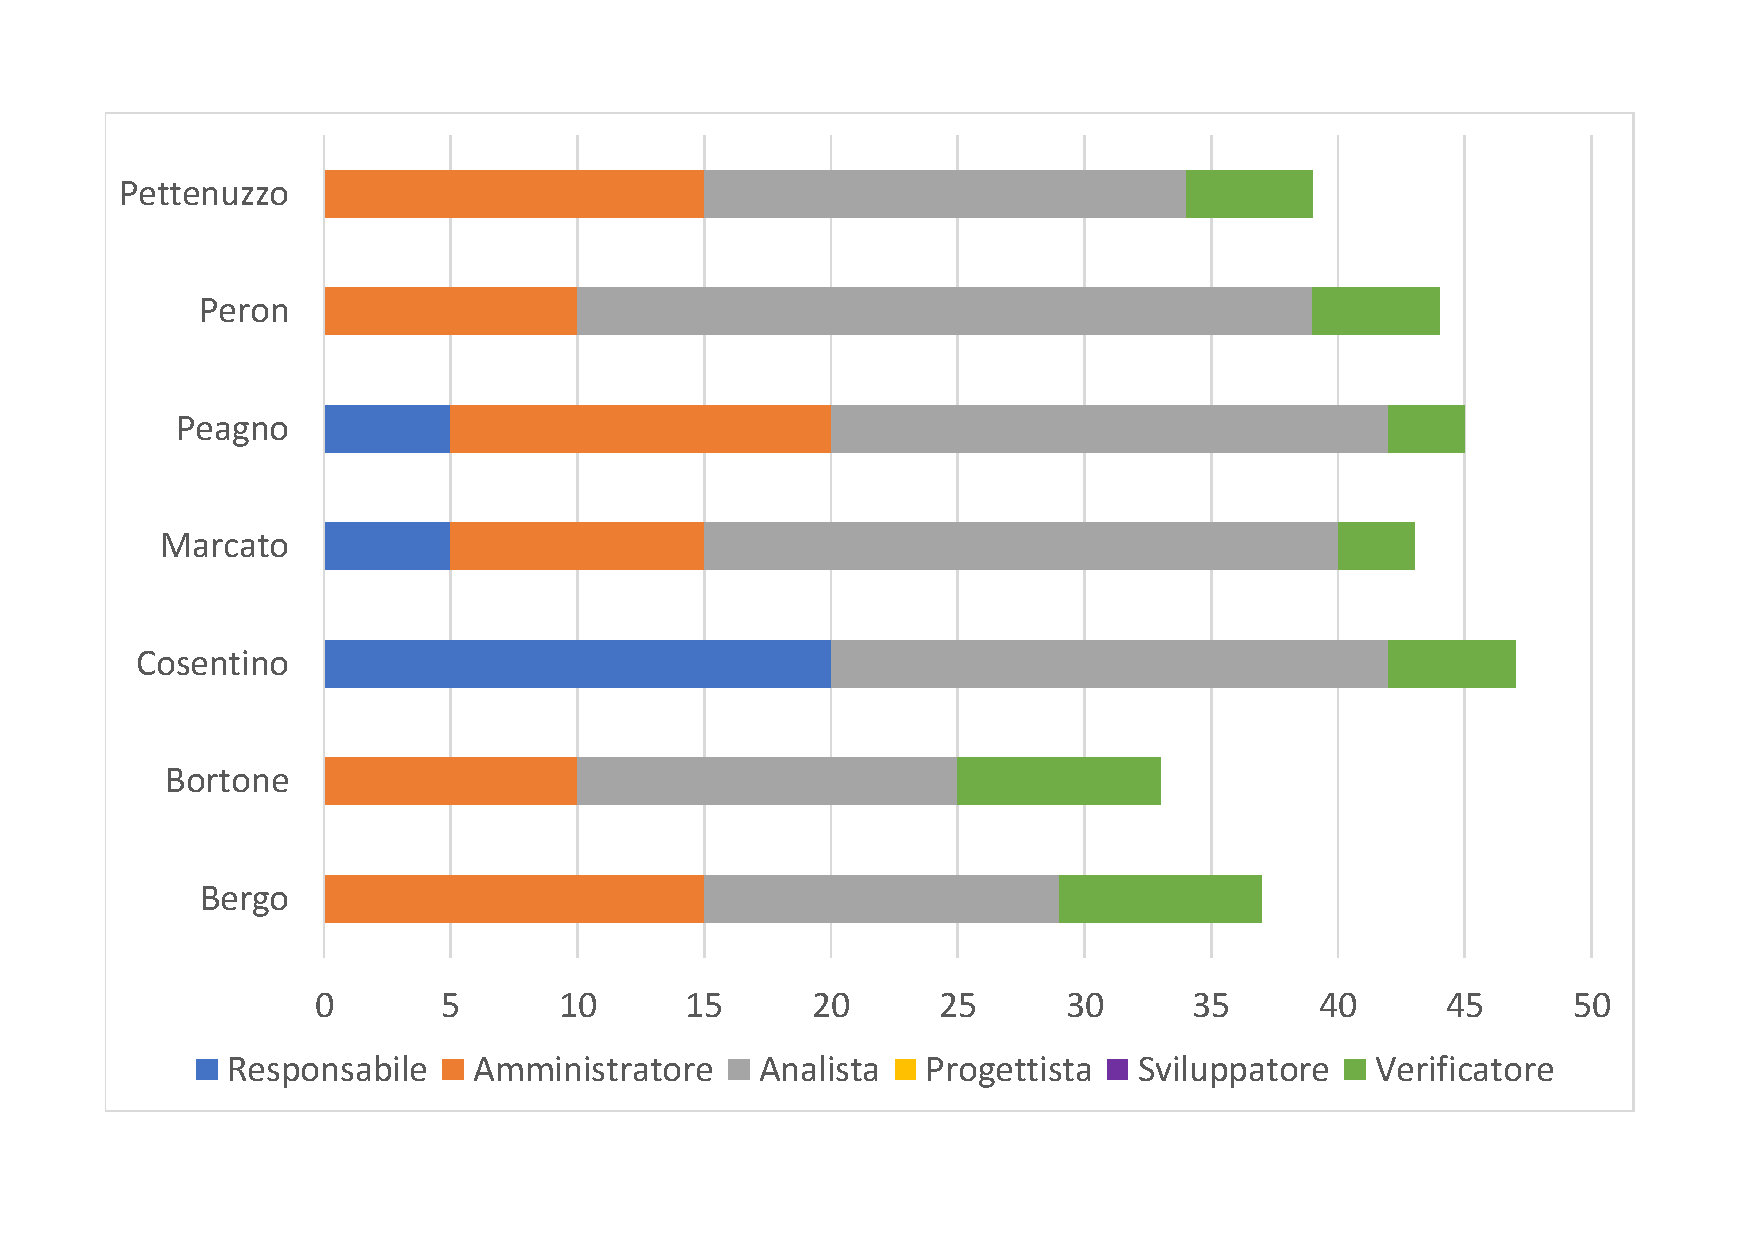
\includegraphics[scale=0.45]{images/preventivoRR.pdf}
	\caption{Istogramma del preventivo della fase 1}
\end{figure}
		
	\subsubsection{Costo}
		Le seguenti tabelle indicano i costi in base ai membri e in base ai ruoli:
		\begin{table}[H]
			\centering		
			\begin{tabular}{| l | l |}
				\rowcolor{LightBlue}
				\textbf{\color{white}Membro}
				& \textbf{\color{white}Costo}\\
			
				Bergo 				& 770€\\
				Bortone 			& 695€\\
				Cosentino 		& 1225€\\
				Marcato 			& 1020€\\
				Peagno 			& 1045€\\
				Peron 				& 1000€\\
				Pettenuzzo 	& 850€\\ \hline
				\textbf{Totale} & 6605€\\ \hline
			\end{tabular}
			\caption{Costo di ciascun membro nella fase 1}
		\end{table}
		
		\begin{table}[H]
			\centering		
			\begin{tabular}{| l | l |}
				\rowcolor{LightBlue}
				\textbf{\color{white}Ruolo}
				& \textbf{\color{white}Costo}\\
			
				Responsabile 		& 900€\\
				Amministratore 	& 1500€\\
				Analista 				& 3650€\\			
				Progettista 			& 0€\\
				Programmatore 		& 0€\\
				Verificatore 		& 555€\\ \hline
				\textbf{Totale} 	& 6605€\\ \hline
			\end{tabular}
			\caption{Costo di ciascun ruolo nella fase 1}
		\end{table}
		

\subsection{Fase 2 (2019-01-22 - 2019-03-15)}
	\subsubsection{Ore preventivate}
		La seguente tabella indica le ore di lavoro per ciascun membro e per ciascun ruolo:
		\begin{table}[H]
			\centering
			\begin{tabular}{| l | c c c c c c | c |}
				\rowcolor{LightBlue}
				& \multicolumn{7}{c}{\textbf{\color{white}Numero di ore}}	\\
	
				\rowcolor{LightBlue}
				\textbf{\color{white}Membro}
				& \textbf{\color{white}RES}
				& \textbf{\color{white}AMM}
				& \textbf{\color{white}AN}
				& \textbf{\color{white}PRO}
				& \textbf{\color{white}DEV}
				& \textbf{\color{white}VER}
				& \textbf{\color{white}Totali}\\

				Bergo      & - & 5 & - & 15 & 15 & 5 	& 40 \\
				Bortone    & - & - & - & 21 & 14 & - & 35 \\
				Cosentino  & - & - & 5 & 13 & 5 & 5 & 28 \\
				Marcato    & - & 10 & - & 10 & 7 & 5 & 32 \\
				Peagno     & - & 4 & - & 16 & - & 10 & 30 \\
				Peron      & 15 & - & - & 10 & 10 & - & 35 \\
				Pettenuzzo & 15 & - & 10 & 5 & - & - & 30 \\ \hline
			\end{tabular}
			\caption{Ore di lavoro per membro/ruolo della fase 2}
		\end{table}	
	\begin{figure}[H]
	\centering
	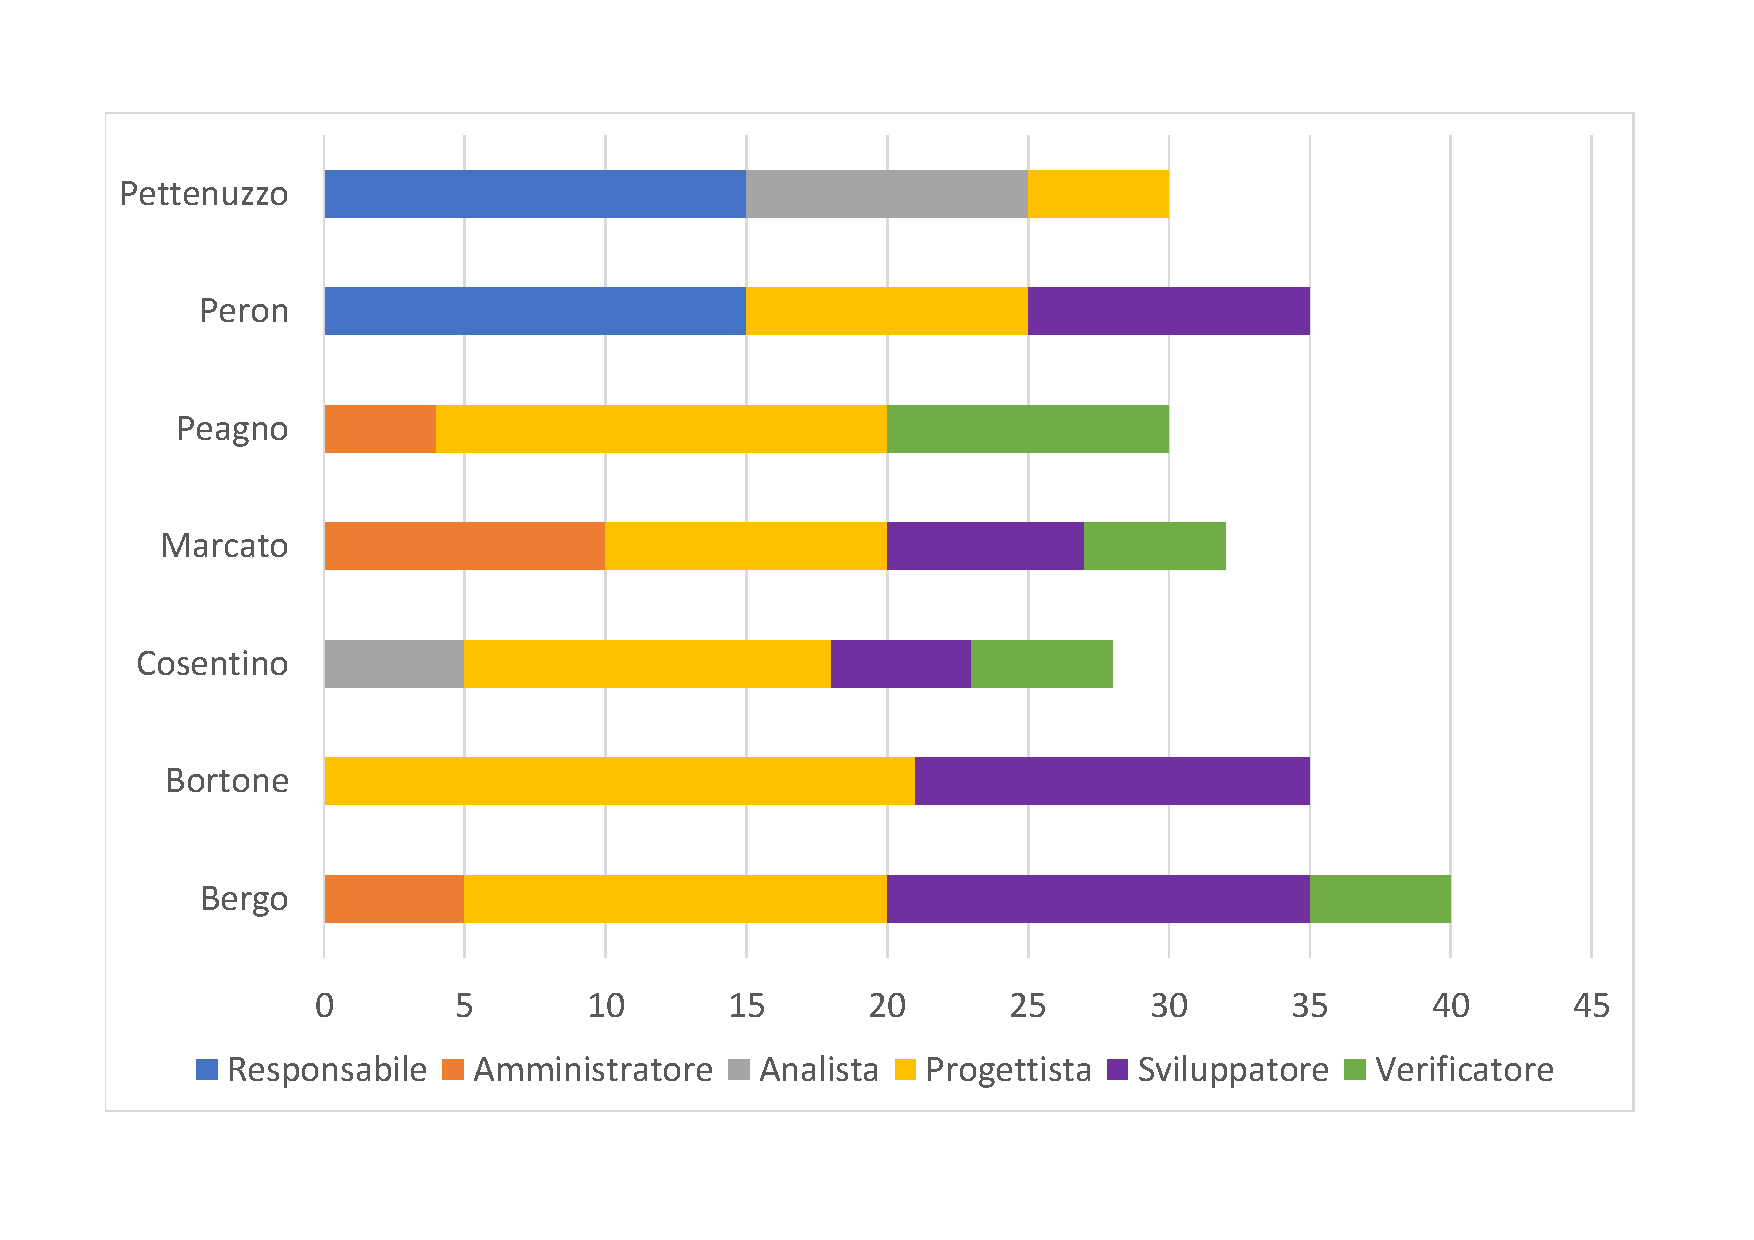
\includegraphics[scale=0.45]{images/preventivoRP.pdf}
	\caption{Istogramma del preventivo della fase 2}
\end{figure}	
		
	\subsubsection{Costo}
		Le seguenti tabelle indicano i costi in base ai membri e in base ai ruoli:	
		\begin{table}[H]
			\centering
			\begin{tabular}{| l | l |}
				\rowcolor{LightBlue}
				\textbf{\color{white}Membro}
				& \textbf{\color{white}Costo}\\
			
				Bergo				& 730€\\
				Bortone			& 672€\\
				Cosentino		& 561€\\
				Marcato			& 600€\\
				Peagno				& 582€\\
				Peron				& 820€\\
				Pettenuzzo		& 810€\\ \hline
				\textbf{Totale} & 4775€\\ \hline
			\end{tabular}
			\caption{Costo di ciascun membro nella fase 2}
		\end{table}
		
		\begin{table}[H]
			\centering
			\begin{tabular}{| l | l |}
				\rowcolor{LightBlue}
				\textbf{\color{white}Ruolo}
				& \textbf{\color{white}Costo}\\
			
				Responsabile 		& 900€\\
				Amministratore 	& 380€\\
				Analista 				& 375€\\			
				Progettista 			& 1980€\\
				Programmatore 		& 765€\\
				Verificatore 		& 375€\\ \hline
				\textbf{Totale} 	& 4775€\\ \hline
			\end{tabular}		
			\caption{Costo di ciascun ruolo nella fase 2}
		\end{table}
		
\subsection{Fase 3 (2019-03-16 - 2019-04-19)}
	\subsubsection{Ore preventivate}
		La seguente tabella indica le ore di lavoro per ciascun membro e per ciascun ruolo:
		\begin{table}[H]
			\centering
			\begin{tabular}{| l | c c c c c c | c |}
				\rowcolor{LightBlue}
				& \multicolumn{7}{c}{\textbf{\color{white}Numero di ore}}	\\
	
				\rowcolor{LightBlue}
				\textbf{\color{white}Membro}
				& \textbf{\color{white}RES}
				& \textbf{\color{white}AMM}
				& \textbf{\color{white}AN}
				& \textbf{\color{white}PRO}
				& \textbf{\color{white}DEV}
				& \textbf{\color{white}VER}
				& \textbf{\color{white}Totali}\\
	
				Bergo      & 15 & - & - & 10 & 10 & 10 & 45 \\
				Bortone    & 15 & - & 5 & 8 & 7 & 10 & 45  \\
				Cosentino  & - & 5 & - & 21 & 21 & - & 47 \\
				Marcato    & - & - & - & 25 & 25 & - & 50 \\
				Peagno     & - & - & - & 25 & 25 & - & 50 \\
				Peron      & - & - & - & 15 & 15 & 15 & 45 \\
				Pettenuzzo & - & - & 5 & 10 & 25 & 10 & 50 \\ \hline
			\end{tabular}
			\caption{Ore di lavoro per membro/ruolo della fase 3}
		\end{table}
		
	\begin{figure}[h]
	\centering
	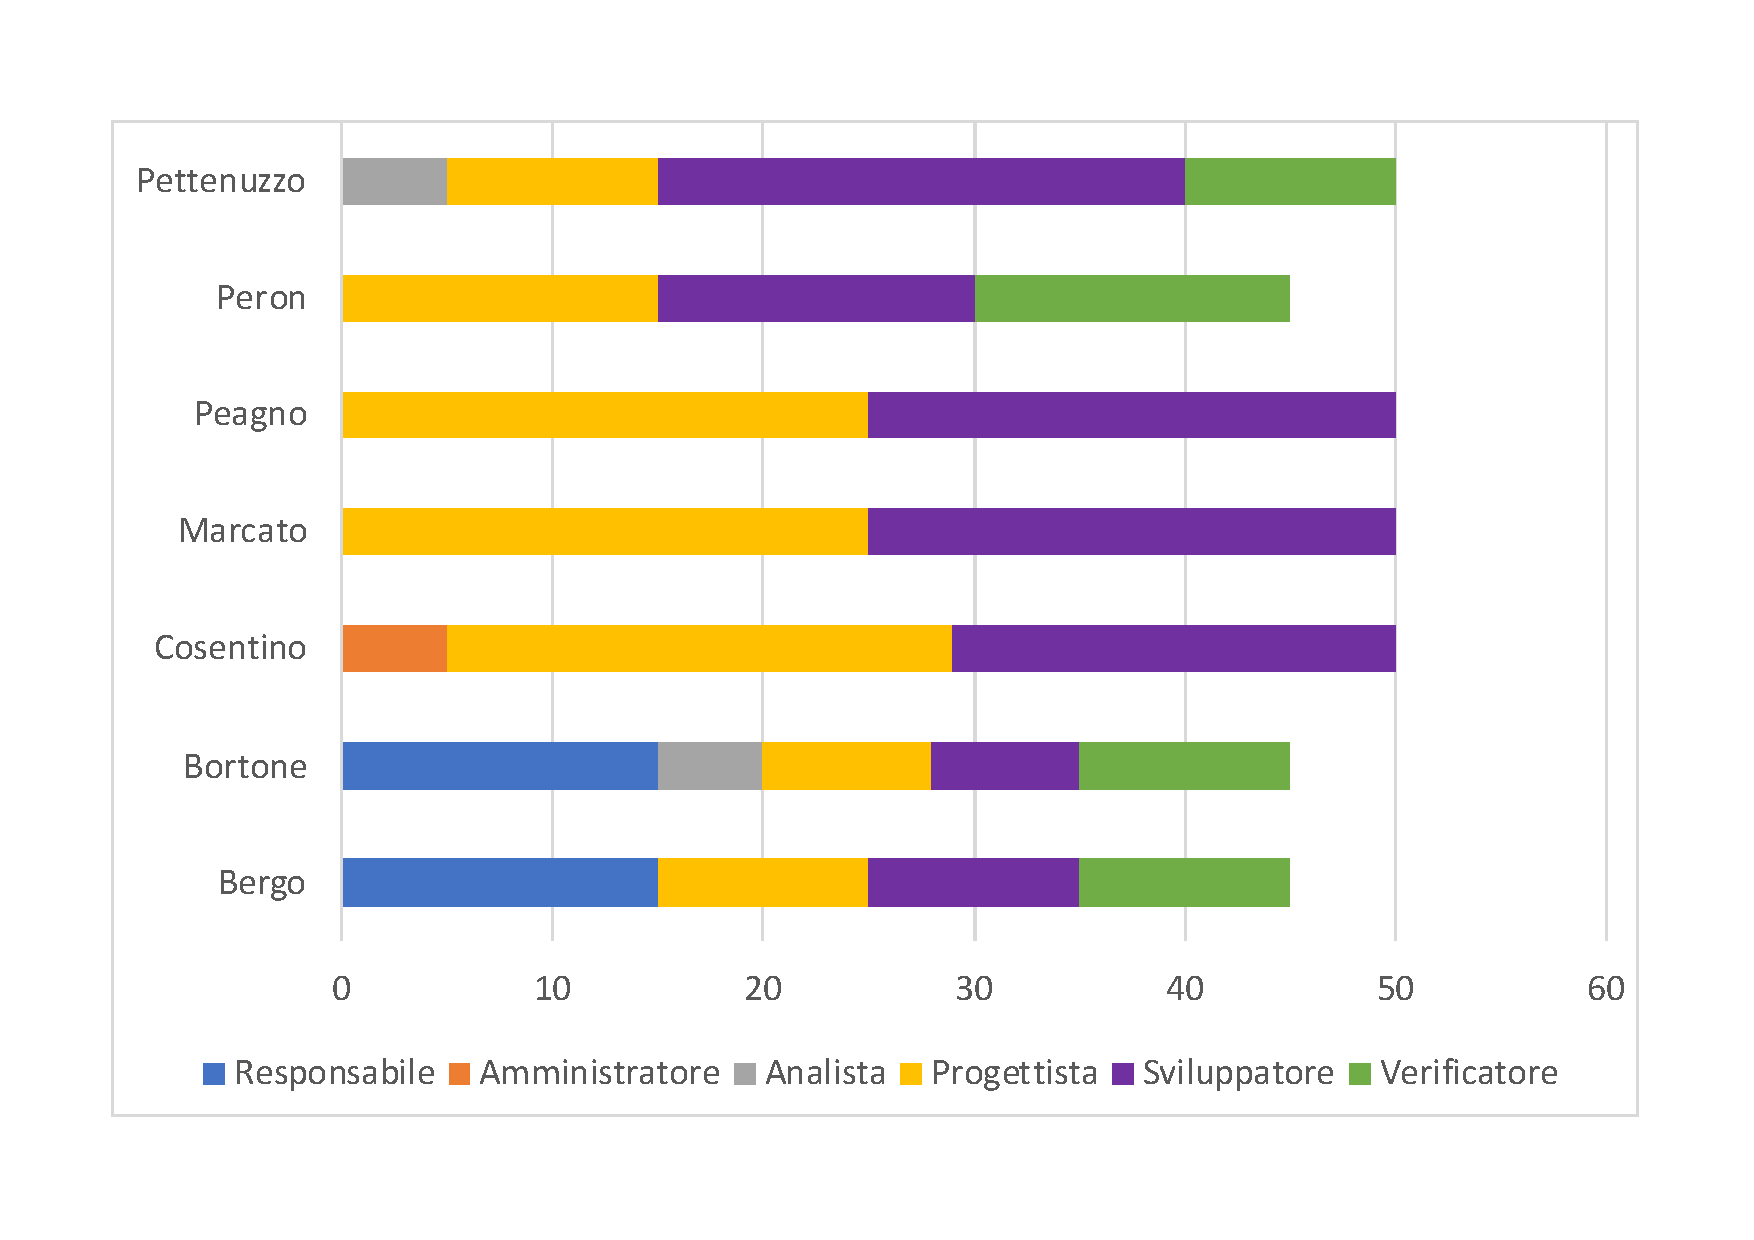
\includegraphics[scale=0.45]{images/preventivoRQ.pdf}
	\caption{Istogramma del preventivo della fase 3}
\end{figure}

	\subsubsection{Costo}
		Le seguenti tabelle indicano i costi in base ai membri e in base ai ruoli:
		\begin{table}[H]
			\centering
			\begin{tabular}{| l | l |}
				\rowcolor{LightBlue}
				\textbf{\color{white}Membro}
				& \textbf{\color{white}Costo}\\
				
				Bergo 				& 970€\\
				Bortone 			& 1006€\\
				Cosentino 		& 877€\\
				Marcato 			& 925€\\
				Peagno 			& 925€\\
				Peron 				& 780€\\
				Pettenuzzo 	& 870€\\ \hline
				\textbf{Totale} & 6353€\\ \hline
			\end{tabular}
			\caption{Costo di ciascun membro nella fase 3}
		\end{table}
		
		\begin{table}[H]
			\centering
			\begin{tabular}{| l | l |}
				\rowcolor{LightBlue}
				\textbf{\color{white}Ruolo}
				& \textbf{\color{white}Costo}\\
				
				Responsabile 		& 900€\\
				Amministratore 	& 100€\\
				Analista 				& 250€\\			
				Progettista 			& 2508€\\
				Programmatore 		& 1920€\\
				Verificatore 		& 675€\\ \hline
				\textbf{Totale} 	& 6353€\\ \hline
			\end{tabular}
			\caption{Costo di ciascun ruolo nella fase 3}
		\end{table}
		
\subsection{Fase 4 (2019-04-20 - 2019-05-17)}
	\subsubsection{Ore preventivate}
		La seguente tabella indica le ore di lavoro per ciascun membro e per ciascun ruolo:
		\begin{table}[H]
			\centering
			\begin{tabular}{| l | c c c c c c | c |}
				\rowcolor{LightBlue}
				& \multicolumn{7}{c}{\textbf{\color{white}Numero di ore}}	\\
		
				\rowcolor{LightBlue}
				\textbf{\color{white}Membro}
				& \textbf{\color{white}RES}
				& \textbf{\color{white}AMM}
				& \textbf{\color{white}AN}
				& \textbf{\color{white}PRO}
				& \textbf{\color{white}DEV}
				& \textbf{\color{white}VER}
				& \textbf{\color{white}Totali}\\
	
				Bergo      & - & - & - & 11 & 11 & - & 22\\
				Bortone    & - & - & - & 8 & 8 & 8 & 24\\
				Cosentino  & - & 3 & - & 7 & 7 & 10 & 27\\
				Marcato    & - & - & - & - & 9 & 10 & 19\\
				Peagno     & 15 & - & - & - & 10 & - & 25\\
				Peron      & - & - & - & 5 & 10 & 10 & 25\\
				Pettenuzzo & - & - & - & 15 & - & 8 & 23\\ \hline
			\end{tabular}
			\caption{Ore di lavoro per membro/ruolo della fase 4}
		\end{table}
		
	\begin{figure}[h]
	\centering
	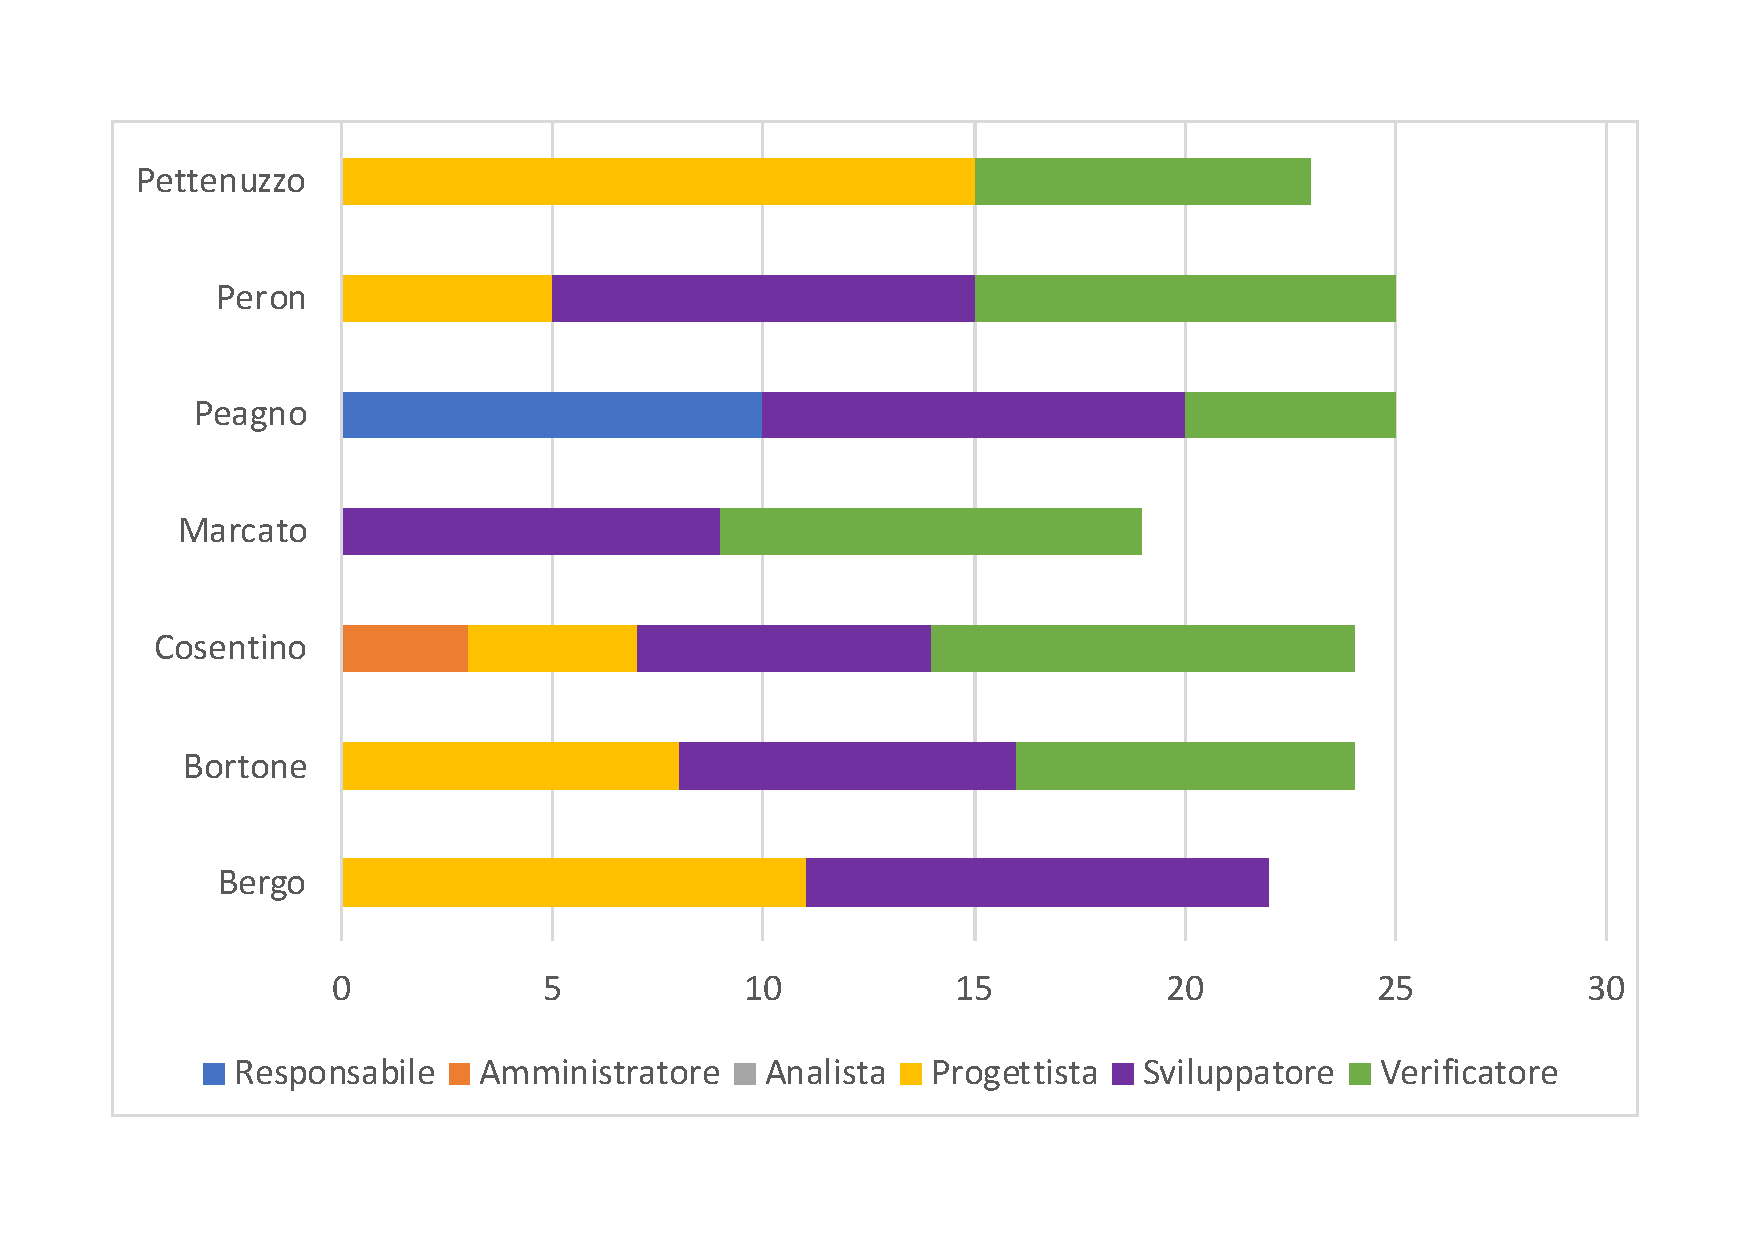
\includegraphics[scale=0.45]{images/preventivoRA.pdf}
	\caption{Istogramma del preventivo della fase 4}
\end{figure}
		
	\subsubsection{Costo}
		Le seguenti tabelle indicano i costi in base ai membri e in base ai ruoli:
		\begin{table}[H]
			\centering
			\begin{tabular}{| l | l |}
				\rowcolor{LightBlue}
				\textbf{\color{white}Membro}
				& \textbf{\color{white}Costo}\\
				
				Bergo				& 407€\\
				Bortone			& 416€\\
				Cosentino		& 469€\\
				Marcato			& 285€\\
				Peagno				& 600€\\
				Peron				& 410€\\
				Pettenuzzo		& 450€\\ \hline
				\textbf{Totale} & 3037€\\ \hline
			\end{tabular}
			\caption{Costo di ciascun membro nella fase 4}
		\end{table}
		
		\begin{table}[H]
			\centering
			\begin{tabular}{| l | l |}
				\rowcolor{LightBlue}
				\textbf{\color{white}Ruolo}
				& \textbf{\color{white}Costo}\\
				
				Responsabile 		& 450€\\
				Amministratore 	& 60€\\
				Analista 				& 0€\\			
				Progettista 			& 1012€\\
				Programmatore 		& 825€\\
				Verificatore 		& 690€\\ \hline
				\textbf{Totale} 	& 3037€\\ \hline
			\end{tabular}		
			\caption{Costo di ciascun ruolo nella fase 4}
		\end{table}

\subsection{Riepilogo}
	\subsubsection{Ore totali}
		La seguente tabella indica le ore di lavoro per ciascun membro e per ciascun ruolo. Tra parentesi vengono indicate le ore totali considerando anche l'investimento. Le ore rendicontate sono quelle delle fasi 2, 3 e 4. La fase 1 è da considerare come investimento per il progetto.
		\begin{table}[H]
			\centering
			\begin{tabular}{| l | c c c c c c | c |}
				\rowcolor{LightBlue}
				& \multicolumn{7}{c}{\textbf{\color{white}Numero di ore}}	\\
		
				\rowcolor{LightBlue}
				\textbf{\color{white}Membro}
				& \textbf{\color{white}RES}
				& \textbf{\color{white}AMM}
				& \textbf{\color{white}AN}
				& \textbf{\color{white}PRO}
				& \textbf{\color{white}DEV}
				& \textbf{\color{white}VER}
				& \textbf{\color{white}Totali}\\
		
				Bergo 				& 15 (15) & 5 (20)		& 0 (14)	& 36 (36) & 36 (36) & 10 (18)	& 102 (139)\\
				Bortone 			& 15  (15)  & 0 (10)		& 5	 (20)	& 37 (37) & 29 (29) & 18 (26)	& 104 (137)\\
				Cosentino 		& 0  (20) & 8 (8)		& 5 (27)	& 41 (41) & 33 (33) & 15  (20)	& 102 (149)\\
				Marcato 			& 0 (5) & 10 (20)		& 0  (25)	& 35 (35) & 41 (41) & 15 (18)	& 101 (144)\\
				Peagno 			& 15  (20) & 4 (19)		& 0  (22)	& 41 (41) & 35 (35) & 10 (13)	& 105 (150)\\
				Peron 				& 15 (15) & 0 (10)		& 0  (29)	& 30 (30) & 35 (35) & 25  (30)	& 105 (149)\\
				Pettenuzzo 	& 15 (15) & 0 (15) 	& 15  (34)	& 30 (30) & 25 (25) & 18 (23)	& 103 (142)\\ \hline
			\end{tabular}
			\caption{Ore di lavoro per membro/ruolo di tutto il progetto}
		\end{table}
	
	\subsubsection{Costo totale}
		Le seguenti tabelle indicano i costi con e senza investimento in base ai membri e in base ai ruoli.
		\begin{table}[H]
			\centering
			\begin{tabular}{| l | l | l |}
				\rowcolor{LightBlue}
				\textbf{\color{white}Membro}
				& \textbf{\color{white}Costo con investimento}
				& \textbf{\color{white}Costo preventivato}\\
				
				Bergo				& 2802€ & 2032€\\
				Bortone			& 2789€ & 2094€\\
				Cosentino		& 3132€ & 1907€\\
				Marcato			& 2830€ & 1810€\\
				Peagno				& 3152€ & 2107€\\
				Peron				& 3010€ & 2010€\\
				Pettenuzzo		& 2980€ & 2130€\\ \hline
				\textbf{Totale} & 20695€ & 14090€\\ \hline
			\end{tabular}
			\caption{Costo di ciascun membro per tutto il progetto}
		\end{table}
		
		\begin{table}[H]
			\centering
			\begin{tabular}{| l | l | l |}
				\rowcolor{LightBlue}
				\textbf{\color{white}Ruolo}
				& \textbf{\color{white}Costo con investimento}
				& \textbf{\color{white}Costo preventivato}\\
				
				Responsabile 		& 3150€ & 2225€\\
				Amministratore 	& 2040€ & 540€\\
				Analista 				& 4275€ & 625€\\			
				Progettista 			& 5500€ & 5500€\\
				Programmatore 		& 3510€ & 3510€\\
				Verificatore 		& 2220€ & 1665€\\ \hline
				\textbf{Totale} 	& 20695€ & 14090€\\ \hline
			\end{tabular}		
			\caption{Costo di ciascun ruolo per tutto il progetto}
		\end{table}
		
		\paragraph{Conclusioni\\}
		Il costo totale del progetto con un investimento di 6605 è pari a \textbf{20695€}. Conseguentemente, il costo preventivato è \textbf{14090€}.